\section{Introduction}
% modeling at different scales for SC-FC relationships
The exploration of structure and function relationships is a fundamental scientific inquiry at all levels of biological organization, and the structure-function relationship of the brain is of immense interest in neuroscience. Attempts at mathematical formulations of neuronal activity began with describing currents traveling through a neuron's membranes and being charged via ion channels \cite{hodgkin_quantitative_1952}. Recently, the focus of computational models have expanded from small populations of neurons to macroscale brain networks, which are now available via diffusion-weighted and functional magnetic resonance imaging (dMRI and fMRI) \cite{bullmore_complex_2009}. Using computational tractography on dMRI images, detailed whole brain white-matter tracts, and their connectivity can be obtained, to yield the brain's structural connectivity (SC). Using correlated activation patterns over time in fMRI data reveals functional connectivity (FC) with high spatial resolution. Such high resolution images of the brain also allowed neuroscientists to label the brain according to anatomical or functional regions of interest (ROIs) \cite{Desikan2006, craddock_whole_2012}. Subsequently, efforts in graph-theoretic modeling have emerged as an effective computational tool to study the brain's SC-FC relationship based on the parcellated brains: ROIs become nodes and connectivity strengths become edges on the graph, while dynamical systems describing neuronal activity are played out on this graph structure \cite{bassett_human_2009,bullmore_complex_2009,cao_topological_2014}.

%%% paragraph on what's been done in graphical modeling
Diverse graph based methods have been employed to relate the brain's SC to FC. Particularly, perturbations and evolution of the structural and functional networks have been investigated using both graph theoretical statistics \cite{chatterjee_understanding_2008, bassett_small-world_2006, he_structural_2008, buckner_molecular_2005, brunel_dynamics_2000, brunel_effects_2001, suarez_linking_2020} as well as network controllability \cite{gu_controllability_2015, muldoon_stimulation-based_2016}. Structurally informed models use graphical representations of the brain's connections to couple anatomically connected neuronal assemblies \cite{Wilson1972, el_boustani_master_2009}, numerical simulations of such neural mass models (NMMs) provides an approximation of the brain's local and global activities, and are able to achieve moderate correlation between simulated and empirical FC \cite{Nunez1974, jirsa_derivation_1997, Valdes1999, honey_predicting_2009, Spiegler2013}. However, approximations through stochastic simulations are unable to provide a closed form solution and inherits interpretational challenges since dynamics is only obtained from iterative optimizations of high dimensional NMM parameters. 

An emergent field of work have suggested low-dimensional processes involving diffusion or random walks on the structural graph as a simple means of simulating FC from SC. These simpler models are equally if not more successful at simulating fMRI FC patterns \cite{abdelnour_network_2014, Atasoy2016} as well as MEG oscillatory patterns \cite{tewarie_how_2019, Raj2020} than conventional NMMs. Lastly, these simpler graph diffusion models, which naturally employ the Laplacian of SC, have been generalized to yield spectral graph models whereby Laplacian eigen-spectra were sufficient to reproduce functional patterns of brain activity, using only a few eigenmodes \cite{Abdelnour2018, Atasoy2016, Raj2020}. Thus, a Laplacian matrix representation of a network can be used to find characteristic properties of the network \cite{Stewart1999}, and its eigenmodes (or spectral basis) are the ortho-normal basis that represent particular patterns on the network. Such spectral graph models are computationally attractive due to low-dimensionality and more interpretable analytical solutions.

%%% paragraph on canonical functional networks + atasoy/ de ville efforts
The SC's Laplacian eigenmodes are therefore emerging as the substrate on which functional patterns of the brain are thought to be established via almost any reasonable process of network transmission \cite{Abdelnour2018, Atasoy2016, robinson_eigenmodes_2016}, and metrics quantifying structural eigenmode coupling strength to functional patterns were also recently introduced \cite{preti_decoupling_2019}. These works mainly focused on replicating canonical functional networks (CFNs), which are stable large scale circuits made up of functionally distinct ROIs distributed across the cortex that were extracted by clustering a large fMRI dataset \cite{Yeo2011}. In \cite{Yeo2011} seven CFNs (these are spatial patterns, not to be confused for the entire network of graph of the connectome) were identified. Hence recent graph modeling work has attempted to address whether these canonical patterns can emerge by only looking at the structural connectivity information of the brain.

%%% Introducing our study
Although spectral graph models have been reasonably successful, they leave several important gaps. First, they accommodate only passive spread, hence are incapable of producing oscillating or traveling phenomena, which are critical properties of brain functional activity. Second, they do not incorporate path delays caused by finite axonal conductance speed of activity propagating through brain networks. Third, they are capable of reproducing only deterministic and steady-state features of empirical brain activity, giving a single predicted FC for a given SC. Hence these models cannot easily explain the substantial variability observed amongst individuals, as well as between different recording session of the same individual. This suggests that simplistic spectral graph models will need to be augmented with a set of richer time- or individual-varying features or parameters in order to make them more realistic. Unfortunately, this is a goal that is at variance with the key attraction of these methods - their parsimony and low-dimensionality.

In this study we propose a novel spectral graph approach that is able to produce a far richer range of functional activity and dynamics without compromising on the simplicity and parsimony of the spectral graph model. We hypothesise that the introduction of realistic path delays and axonal conductance speeds can allow graph spectra to display the kinds of pattern-richness observed in real data. Hence we utilize both the SC connectivity strength matrix as measured by white-matter fiber tract density, as well as the distance matrix as measured by the average white-matter fiber tract distance between pairs of ROIs. We show that the additional distance information allows for examining of network dynamics in the complex domain in terms of a novel complex-valued Laplacian. This approach involves only global model parameters, which between them accommodate a rich diversity of spatiotemporal patterns that are capable of closely reproducing the diversity of spatial patterning seen across a large number of healthy subjects. Through this minimalist complex diffusion model, the characteristic patterns of signal spread described by corresponding complex-valued eigen-spectra can be tuned to exhibit activation patterns resembling human CFNs. We show that the complex approach significantly and consistently exceeds the performance of existing works relating real-valued SC Laplacian's eigen-spectra to measured FC \cite{Atasoy2016, preti_decoupling_2019, Abdelnour2018, honey_predicting_2009}. The introduction of the complex-valued Laplacian and accompanying complex graph diffusion may be an important contribution to the emerging literature on graph models of brain activity, and furthers our understanding of the structure-function relationship in the human brain.

We begin with a general theory of complex graph diffusion incorporating path delays, leading to the emergence of the complex-valued Laplacian. Then we present detailed statistical analysis showing the ability of complex eigenmodes to be tuned by model parameters and reproducing CFNs. We present comparison with the current approach of using real-valued eigenmodes, followed by a detailed Discussion.

\section{Theory}
\label{sec:theory}

\paragraph{Notation.} In our notation, vectors and matrices are represented in \textbf{bold}, and scalars by normal font. We denote frequency of a signal, in Hertz (Hz), by symbol $f$, and the corresponding angular frequency as $\omega = 2 \pi f$. The structural connectivity matrix is denoted by $\bm{C} = c_{l,m}$, consisting of connection strength $c_{l,m}$ between any two pairs of brain regions $l$ and $m$.


\subsection{Network Diffusion of Brain Activity}
For an undirected, weighted graph representation of the structural network $c_{l,m}$, we model the average neuronal activation rate for the $l$-th region as $x_{l}(t)$:

\begin{equation} 
    \label{eq:eq1}
    \frac{dx_{l}(t)}{dt} = -\beta (x_{l}(t) - \alpha \sum_{l \ne m}^{m} c_{l,m} x_{m}(t-\tau^{\nu}_{l,m})) + p_{l}(t)
\end{equation}

Where we have a mean firing rate equation at the $m$-th region controlled by an inverse of the common characteristic time constant $\beta$, and input signals from the $l$-th regions connected to region $m$ are scaled by the connection strengths from $c_{m,l}$ and delayed by $t-\tau^{\nu}_{m,l}$. The term $\tau^{\nu}_{m,l}$ is the delay in seconds obtained from the distance adjacency matrix defined by $\tau^{\nu}_{m,l} = \frac{D_{m,l}}{\nu}$, with $\nu$ representing the conductance speed in the brain's SC network. The global coupling parameter $\alpha$ acts as a controller of weights given to long-range white-matter connections.

The delays between connected brain regions turn into phase shifts in the frequency profiles of the oscillating signals. Thus we obtain the following Fourier transforms from (\ref{eq:eq1}): $\frac{dx_{l}(t)}{dt} \to j\omega X_{l}(\omega)$, $x(t-\tau^{\nu}_{m,l}) \to e^{-j\omega \tau^{\nu}_{m,l}} X_{m}(\omega)$, and the oscillatory frequency $\omega = 2 \pi f$. Applying the listed Fourier transforms to (\ref{eq:eq1}) we can obtain the following:

\begin{equation}
    \label{eq:eq2}
    j\omega X_{l}(\omega) = -\beta (X_{l}(\omega) - \alpha \sum_{m \ne l}{c_{m,l}X_{m}(\omega)\exp{-j \omega \tau^{\nu}_{m,l}}}) + p_{l}(\omega)\\
\end{equation}

We then define a complex connectivity matrix as a function of angular frequency $\omega$ as $\pmb{C}^{*}(\omega)={c_{m,l}\exp{-j \omega \tau^{\nu}_{m,l}}}$. Therefore, a structural connectivity matrix whose nodes are normalized by $\deg_{m} = \sum_{l} c_{ml}$ at frequency $\omega$ can be expressed as:

\begin{equation}
    \label{eq:eq3}
    \pmb{C}(\omega) = diag(\frac{1}{\pmb{\deg}}) \pmb{C}^{*}(\omega)
\end{equation}

Replacing the connectivity term in (\ref{eq:eq2}) with (\ref{eq:eq3}) and adjusting all vector notations into matrix notation, we derive the following equations for network level activity in the frequency domain:

\begin{equation}
    \label{eq:eq4}
    j\omega \pmb{X}(\omega) = -\beta (\pmb{X}(\omega) - \alpha \pmb{X}(\omega) \pmb{C}(\omega)) + \pmb{P}(\omega)
\end{equation}


\begin{equation}
    \label{eq:eq5}
    \pmb{X}(\omega)(j\omega \pmb{I} + \beta (\pmb{I} - \alpha \pmb{C}(\omega)))=  \pmb{P}(\omega)
\end{equation}

\subsection{Complex Laplacian Matrix}
Our goal is to examine the characteristic patterns of diffusion revealed by the structural network's normalized Laplacian matrix. Here, we make use of (\ref{eq:eq3}) to introduce a complex Laplacian matrix that absorbs the network properties of both the structural connectivity matrix as well as the distance adjacency matrix. By substituting the complex Laplacian matrix and rebalancing (\ref{eq:eq5}), we obtain a closed-form solution for $\pmb{\bar{X}}(\omega)$:

% have closed form solution wih X(\omega) on one side
\begin{equation}
\label{eq:eq6}
\pmb{X}(\omega) = (j \omega I + \beta \mathcal{L}(\alpha, k))^{-1} \pmb{P}(\omega)
\end{equation}

In this closed-form solution, we defined a complex Laplacian matrix $\mathcal{L}$ as a function of global coupling strength $\alpha$ and wave number $k$, which facilitates the dynamics and frequency profiles observed on the brain's connectome. Since frequency $\omega$ and transmission speed $\nu$ always occur as a ratio, we define the wave number $k = \frac{\omega}{\nu}$. The wave number represents the spatial frequency of any propagating wave, describing the amount of oscillations per unit distance traveled \cite{French1971}. Then the complex Laplacian matrix $\mathcal{L}$ has the form:

\begin{equation}
    \label{eq:eq7}
    \mathcal{L}(\alpha, k) = \pmb{I} - \alpha \pmb{C}^{*}(k)
\end{equation}

Where $\pmb{I}$ is the identity matrix and $\pmb{C}^{*}(k)$ is the complex connectivity matrix as defined above. While (\ref{eq:eq3}) indicates that the propagating signals in the network is governed by $\mathcal{L}$, the complex Laplacian of the network describes the characteristic patterns of signal spread in a network, and we can obtain these spatial patterns via the decomposition:

\begin{equation}
\label{eq:eq8}
\bm{\mathcal{L}}(\alpha, k) = \sum_{n = 1}^{N} \bm{u}_{n}(\alpha, k)\lambda_{n}(\alpha, k)\bm{u}_{n}^{H}(\alpha, k)
\end{equation}

Where $\lambda_{n}(\alpha, k)$ are the eigenvalues of the complex Laplacian matrix and $\bm{u}_{n}(\alpha, k)$'s are the complex eigenmodes of the complex Laplacian matrix. Here, the entries of the complex Laplace eigenmodes represent the relative amount of activation in each parcellated brain region as controlled by global coupling and wave number parameters.

\begin{figure}[ht!]
  \centering
  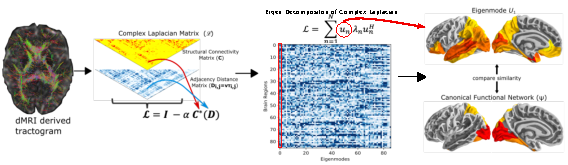
\includegraphics[width=\textwidth]{../figures/chapter4/fig1_overview_v4.pdf}
  \caption{The analysis overview. Structural connectivity matrix ($C$) and distance adjacency matrix ($D$) were extracted from diffusion MRI derived tractograms, to construct the complex Laplacian of the brain's structural network. An eigen decomposition on the network's complex Laplacian ($\mathcal{L}$) was performed obtain complex structural eigenmodes of the brain ($U$). The spatial similarities were computed between the structural eigenmodes and canonical functional networks in fMRI. Here, as an example, we show brain rendering of the leading eigenmode from the HCP template structural connectome (right column, top) and the canonical visual functional network (right column, bottom).}
  \label{fig:fig1}
\end{figure}